\documentclass[11pt]{beamer}
\usepackage[UTF8]{ctex}
\usepackage[utf8]{inputenc}
\usepackage[T1]{fontenc}
\usepackage{lmodern}
\usepackage{amsmath}
\usepackage{amsfonts}
\usepackage{amssymb}
\usepackage{graphicx}
\usetheme{CambridgeUS}

\usepackage{pdfpages}


%%%%%
\usepackage{longtable}
\usepackage{subfigure}
\usepackage{color}
\usepackage{booktabs}

\begin{document}
\author{郭泰彪}
\title{区块链原理及应用}
\subtitle{第2课:区块链的发展历程快速回顾\footnote{不推荐投资加密货币,谨防上当受骗。}}
\logo{
\includegraphics[scale=0.2]{figures/HNUC.jpeg}}
\institute{湖南工商大学大数据研究院}

\begin{frame}[plain]
	\maketitle
\end{frame}

\begin{frame}[shrink]
	\frametitle{目录}
	\tableofcontents[sectionstyle=show,subsectionstyle=show/shaded]
\end{frame}

\section{比特币的燃情岁月}

\subsection{比特币趣事两则}
\begin{frame}{如果大三学生的你有6000元,该投资什么}
	\begin{figure}
		\centering
		{\Huge 如果你有6000元,投资什么?}
	\end{figure}
\end{frame}

\begin{frame}{知乎19982269号问题}

	大三的学生,手头有6000元的钱,想要做些小投资赚点儿钱,有什么好建议么?

	\footnotesize{这是除去学费和生活费之后的,所以觉得就存在银行里没什么用,想利用这些钱去做点投资。}
\end{frame}

\begin{frame}{知乎19982269号问题}
	\begin{figure}
		\centering
		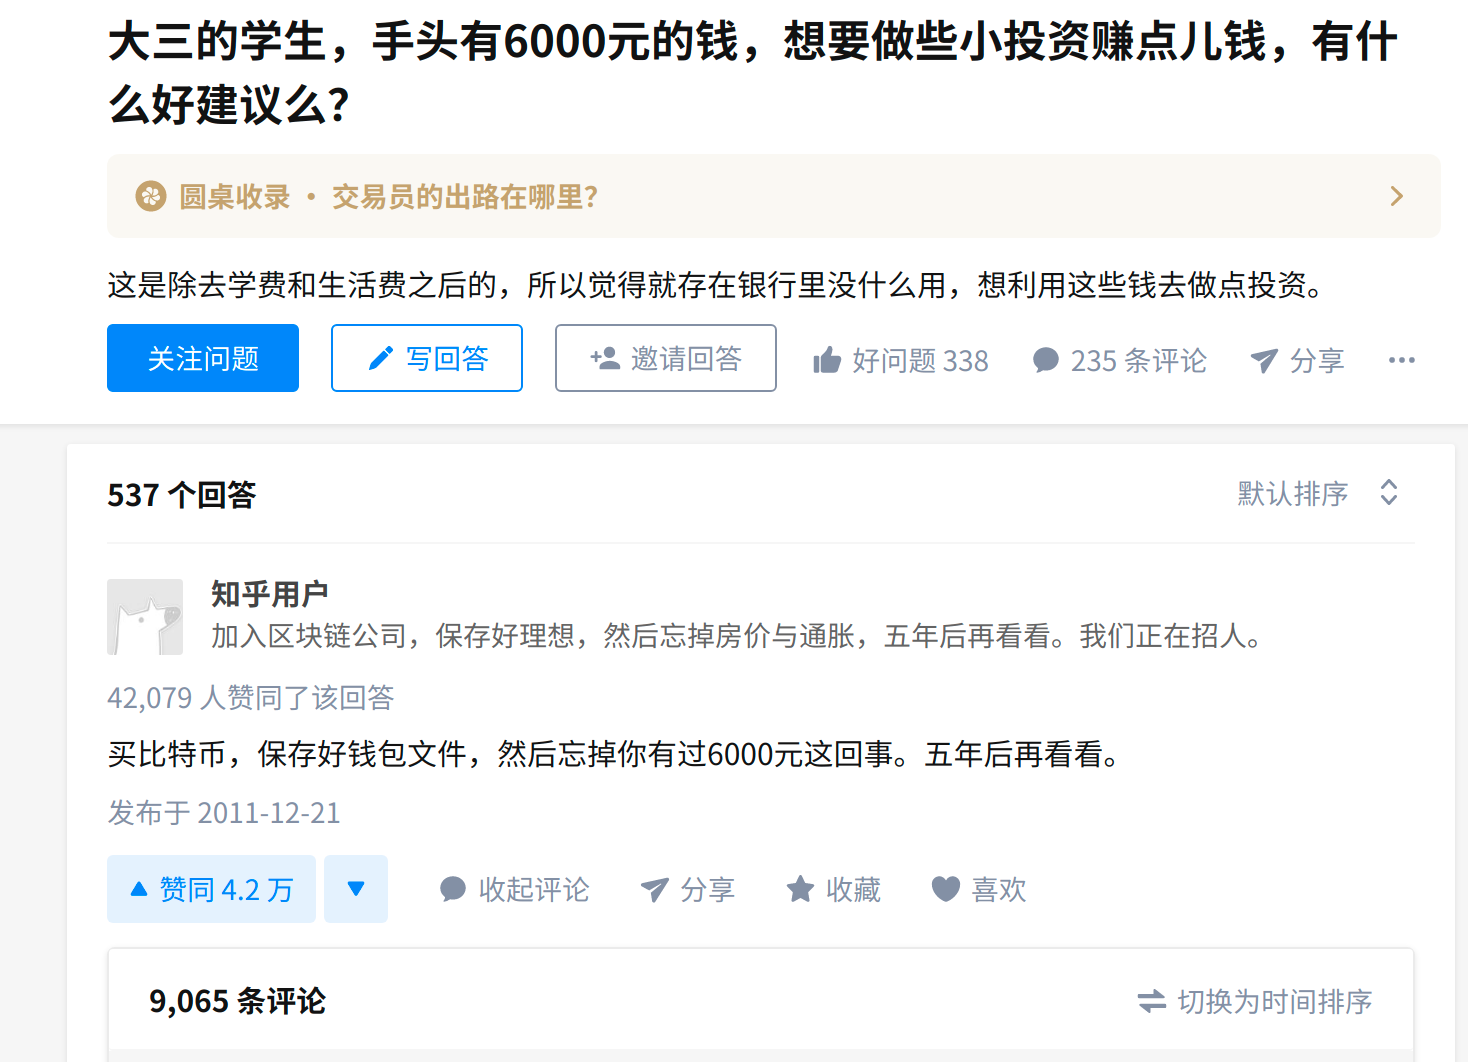
\includegraphics[width=0.8\linewidth]{figures/zhihu19982269}
		\label{fig:zhihu19982269}
	\end{figure}
\end{frame}

\begin{frame}{知乎19982269号问题}
	\begin{figure}
		\centering
		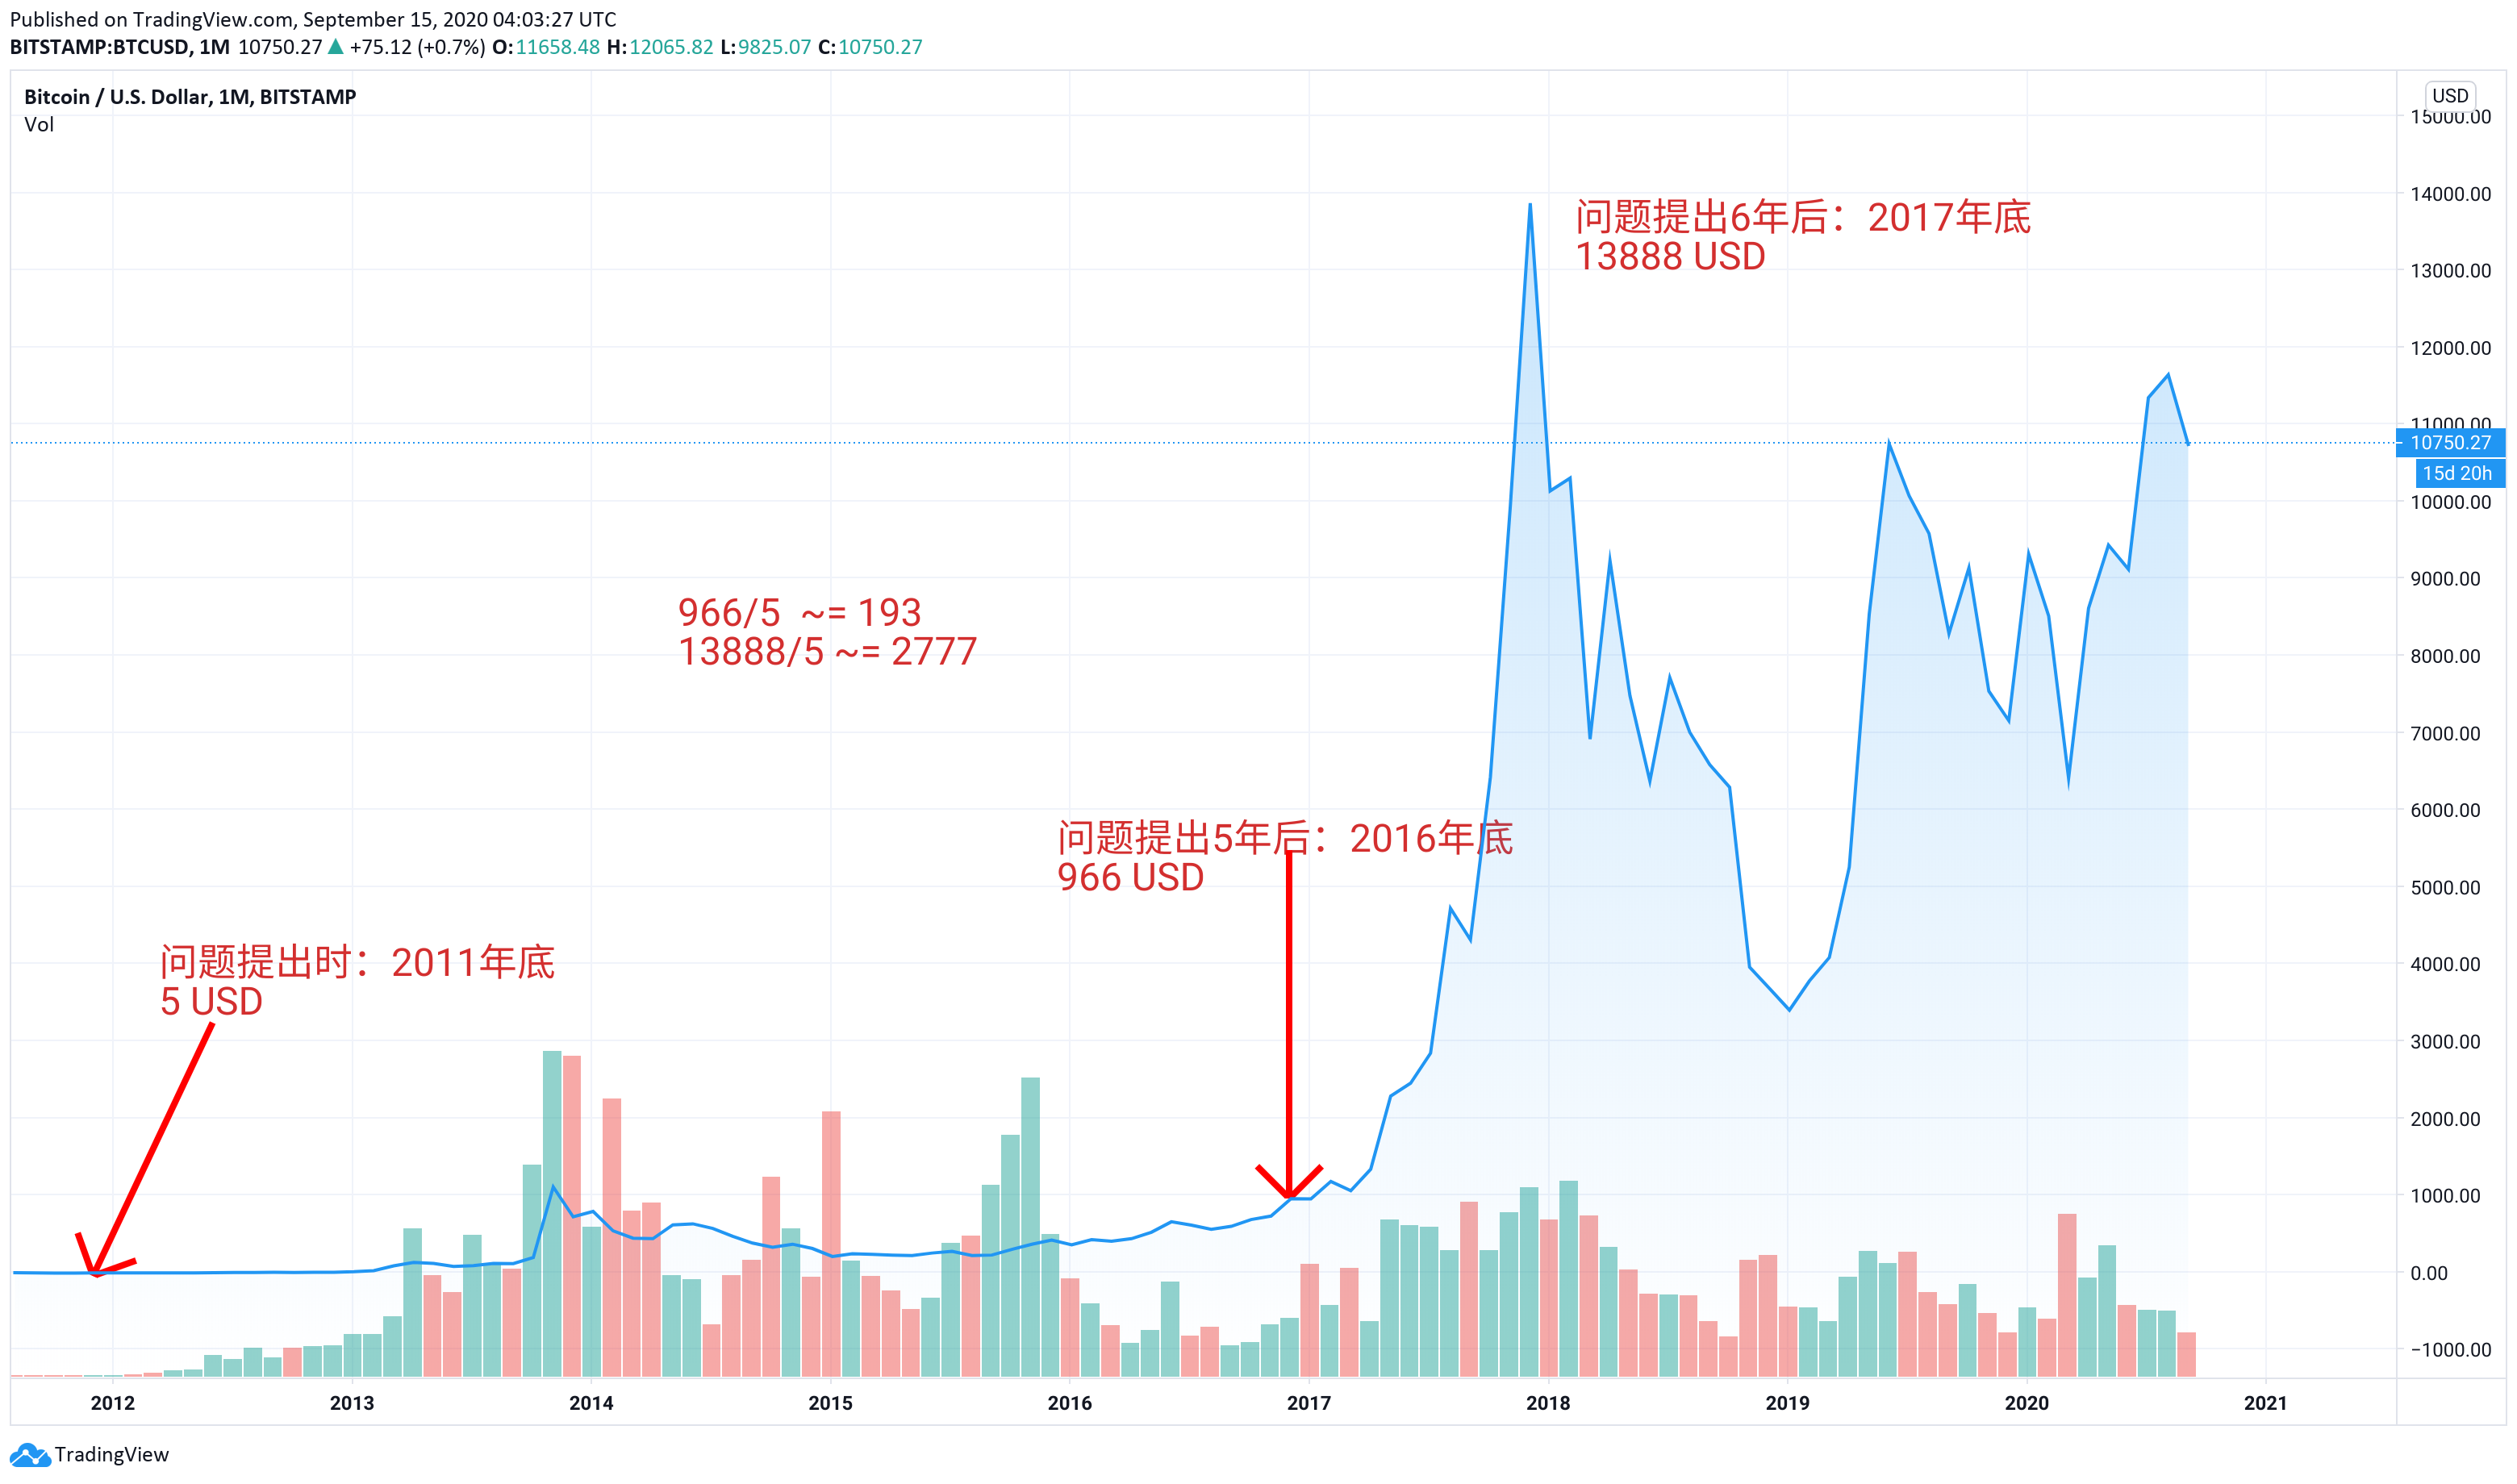
\includegraphics[width=\linewidth]{figures/btc6000}
		\label{fig:zhihu19982269}
	\end{figure}
\end{frame}

\begin{frame}{比特币点外卖,三天才送到}
	翻译: 我想要2块大披萨,希望能用10000枚比特币来换。披萨可以是从商店购买的,也可以是自制的。但是我需要你把披萨送到我的家门口,就像酒店的餐饮服务一样,不需要我自己准备并购买。我喜欢洋葱、胡椒、香肠和蘑菇,不要奇怪的鱼肉披萨!
	\begin{figure}
		\centering
		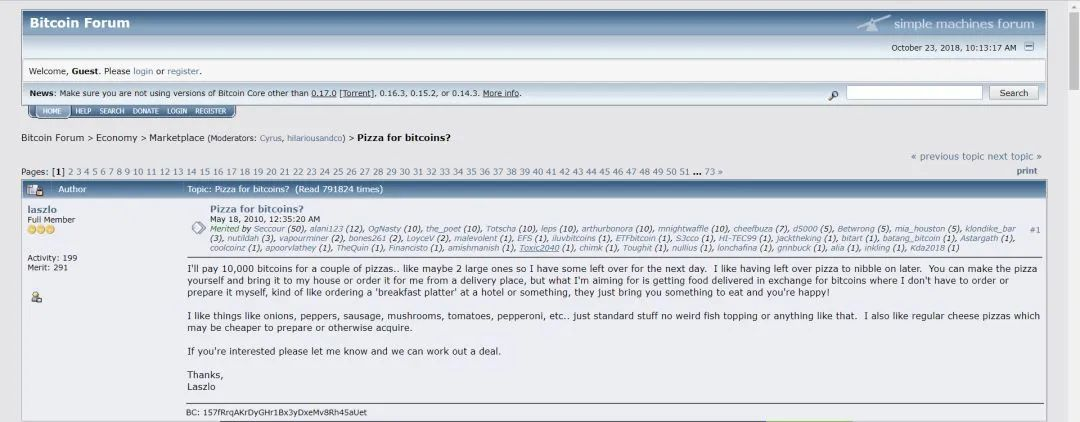
\includegraphics[width=0.7\linewidth]{figures/pizzabbs}
		\caption{比特币论坛帖子截图}
		\label{fig:pizzabbs}
	\end{figure}
\end{frame}

\begin{frame}[allowframebreaks]{Hanyecz买披萨时的截图}
	\begin{figure}
		\centering
		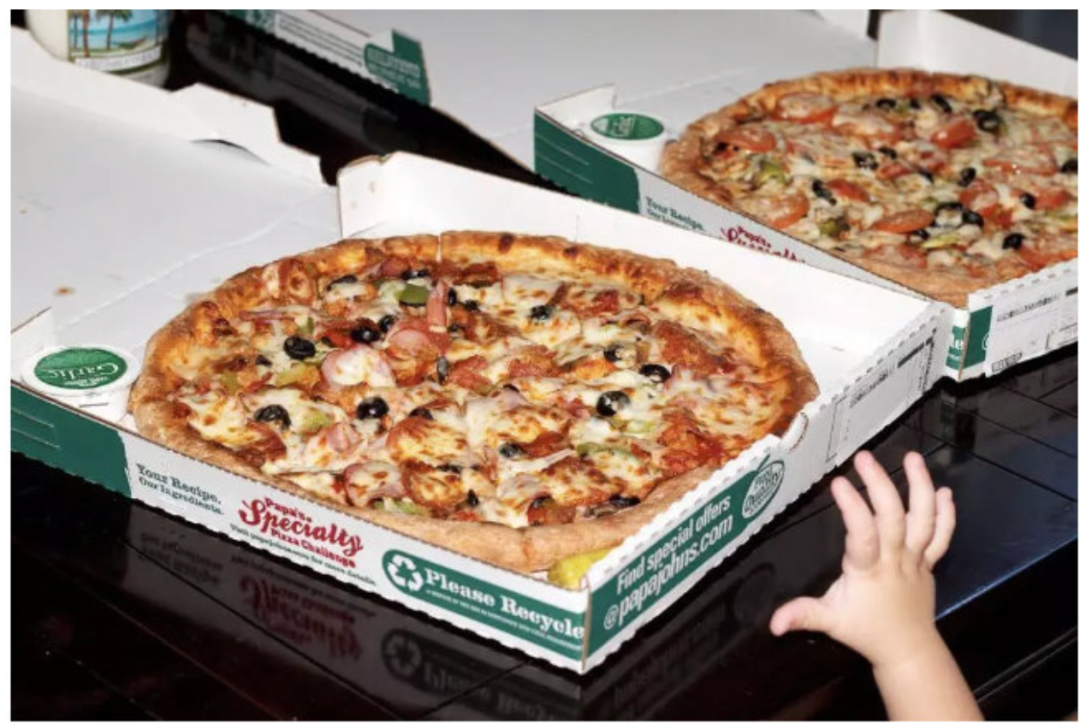
\includegraphics[width=0.7\linewidth]{figures/pizza01}
		\caption{世界上最贵的两块披萨}
	\end{figure}

	\begin{figure}
		\centering
		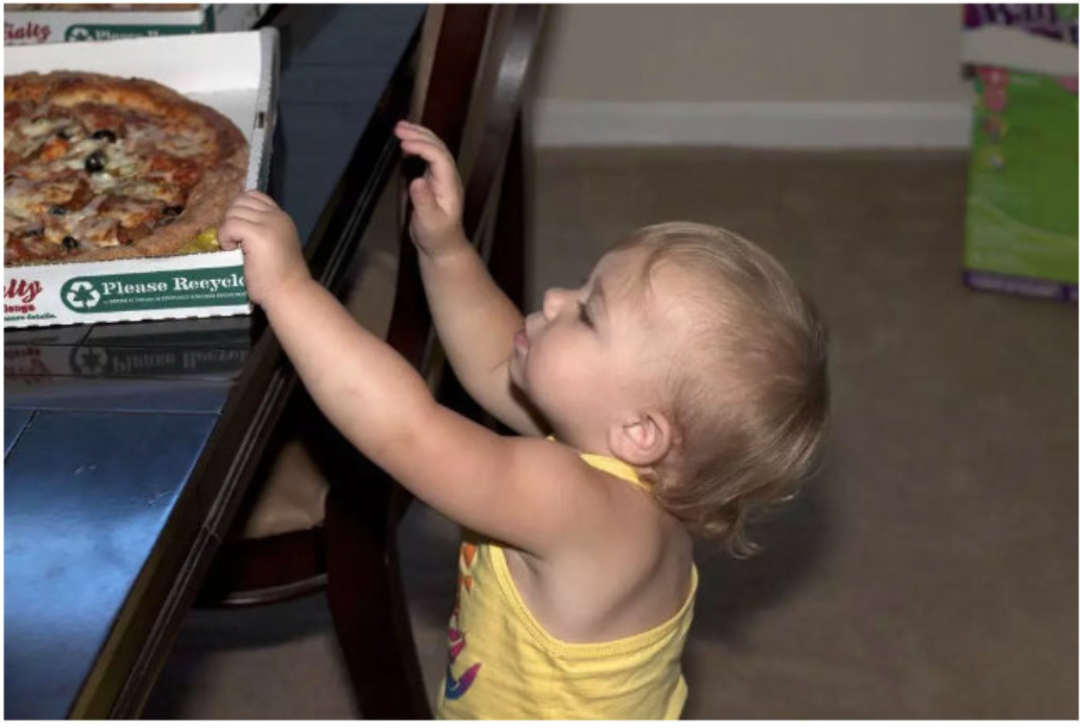
\includegraphics[width=0.7\linewidth]{figures/pizza02}
		\caption{Laszlo表示自己1岁的女儿不是用比特币换的}
	\end{figure}

	\begin{figure}
		\centering
		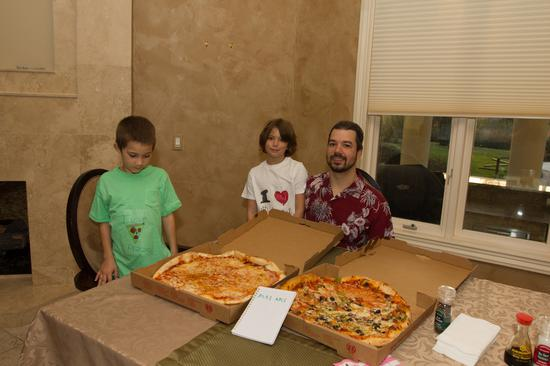
\includegraphics[width=0.6\linewidth]{figures/pizzabybtc}
		\caption{Laszlo在交易完成后还上传了自己与家人共同享用披萨的照片,有趣的是他的一个孩子穿着印有“我爱披萨”字样的衣服,另一个孩子穿着印有“我爱比特币”的衣服}
		\label{fig:pizzabybtc}
	\end{figure}

\end{frame}

\subsection{挖矿的军备竞赛}
\begin{frame}
	Laszlo 为什么拥有这么多比特币?
	
	比特币购买披萨的主人公是GPU挖矿第一人。(2010年)
\end{frame}

\begin{frame}{从CPU到ASIC}
\begin{figure}
	\centering
	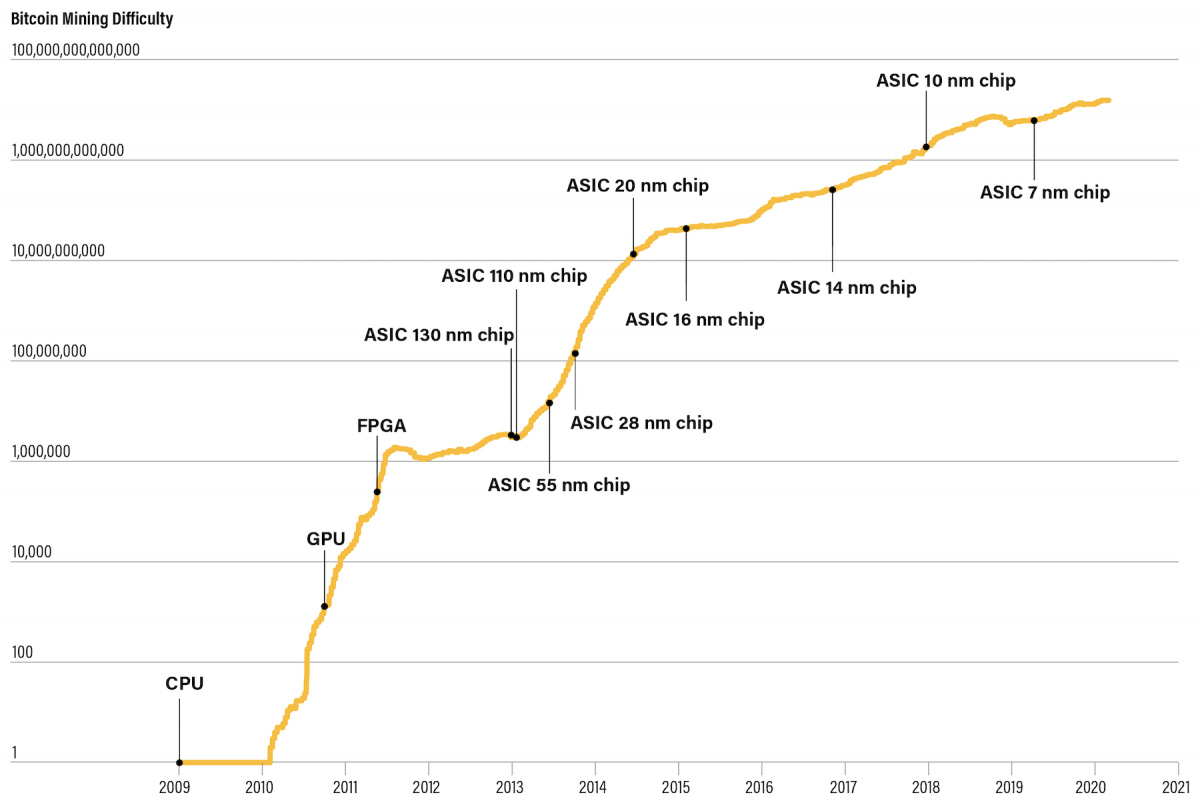
\includegraphics[width=0.8\linewidth]{figures/deviceRevolutionWithPrice}
	\caption{比特币挖矿设备进化速度和比特币挖矿难度关系}
	\label{fig:devicerevolutionwithprice}
\end{figure}
\end{frame}

\begin{frame}{从CPU到ASIC}
	\begin{figure}
		\centering
		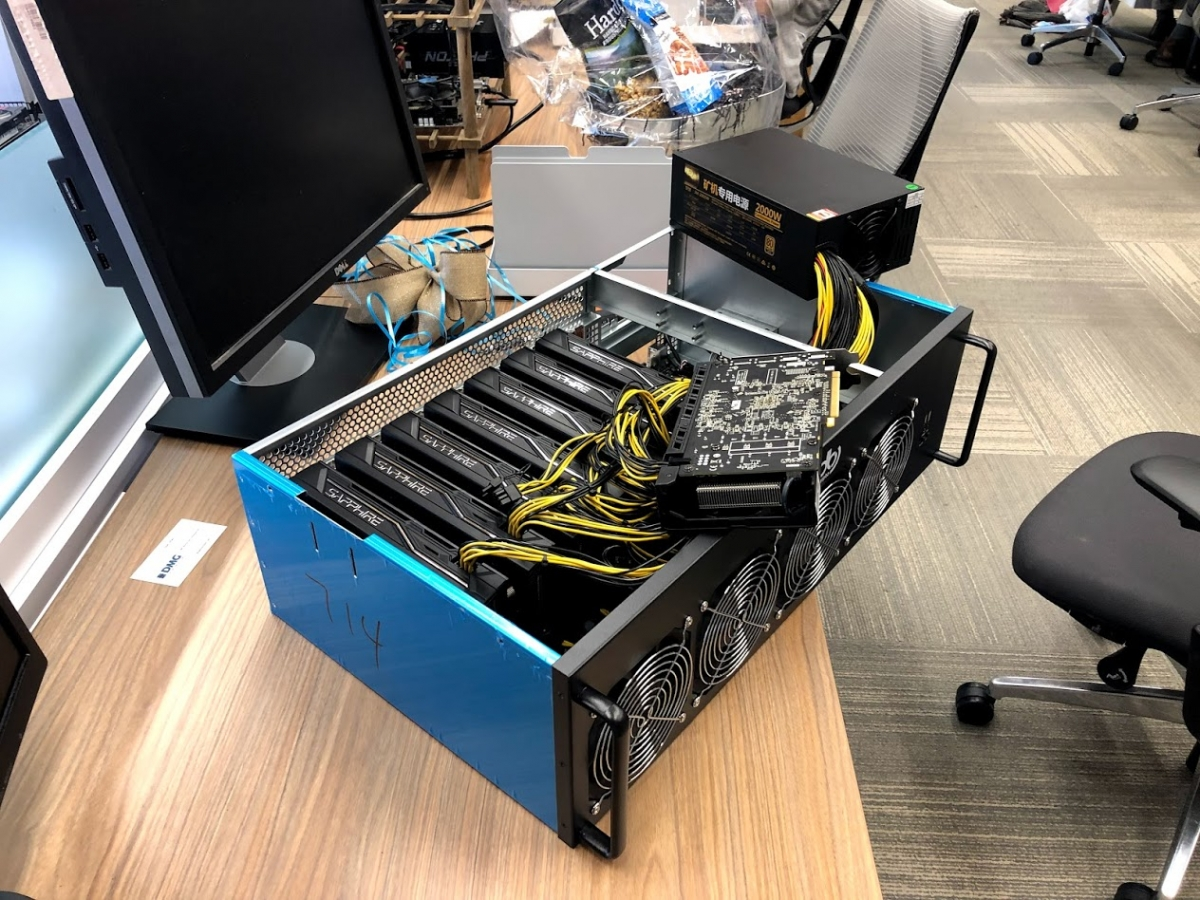
\includegraphics[width=0.7\linewidth]{figures/GPUMining}
		\caption{多路GPU矿机}
	\end{figure}
\end{frame}

\begin{frame}{从CPU到ASIC}
	\begin{figure}
		\centering
		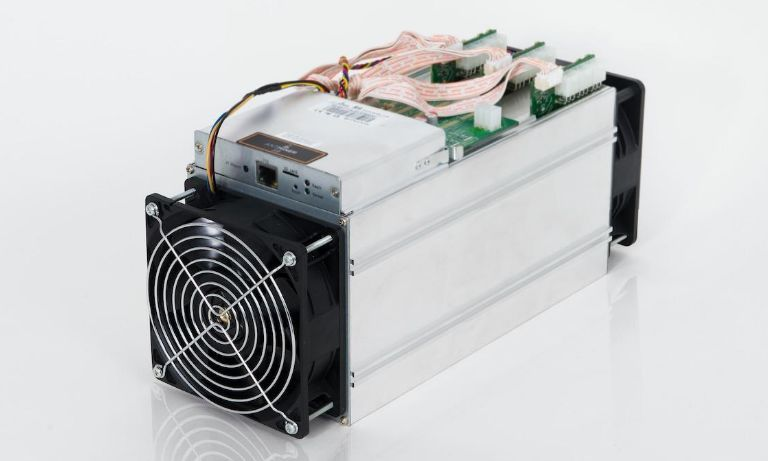
\includegraphics[width=0.7\linewidth]{figures/ASICMining}
		\caption{ASIC矿机}
	\end{figure}
\end{frame}

\begin{frame}{CPU、GPU、FPGA、ASIC挖矿性能对比}

% Please add the following required packages to your document preamble:
% \usepackage{booktabs}
% \usepackage{graphicx}
\begin{table}[]
	\centering
	\resizebox{0.8\textwidth}{!}{%
		\begin{tabular}{@{}p{0.25\linewidth}p{0.25\linewidth}p{0.25\linewidth}p{0.25\linewidth}@{}}
			\toprule
			& CPU            & GPU          & ASIC         \\ \midrule
			适用场景                  & 通用计算           & 半通用计算,适合图像处理 & 专用计算,针对特点算法  \\
			代表产品               & Intel i7 2600k & GTX 1080     & Antminer s9i \\
			价格(\$)              & 316            & 800          & 794          \\
			针对SHA256算法的算力(GH/Z) & 0.02           & 2.8          & 14000        \\
			功耗(W)               & 120            & 300          & 1375         \\
			单位算力功耗(W/GHs)       & 6000           & 107          & 0.098        \\
			单位算力价格(\$/GHs)      & 15800          & 286          & 0.06         \\ \bottomrule
		\end{tabular}%
	}
	\caption{CPU、GPU、ASIC挖矿性能对比\footnote{资料来源:en.bitcoin.it、比特大陆官网、github、国盛证券研究所}}
	\label{tab:my-table}
\end{table}
\end{frame}

\subsection{比特币矿池}
\begin{frame}{单机挖矿到矿池挖矿}
	比特币挖矿规则:大约7分钟出一个区块,某个矿工得到所有的奖励,算力越高的矿工得到奖励的几率越大。两种挖矿的模式:
	\begin{enumerate}
		\item 个人挖矿(Solo):
			\begin{itemize}
				\item 比特币初期流行的挖矿方式;
				\item 但随着比特币挖矿人数变多,算力增加,收益变得不稳定;
			\end{itemize}
		\item 矿池挖矿(Stake Pool):
			\begin{itemize}
				\item 现在比特币主流的挖矿方式;
				\item 将大家算力集中起来,将挖到的比特币进行平分,收益稳定;
			\end{itemize}
	\end{enumerate}
	\begin{align}
		E_{solo}&=E_{stake}\\
	\sigma_{solo}&>=\sigma_{stake}
	\end{align}	
\end{frame}

\begin{frame}{矿池收益结算模式}
	\begin{enumerate}
		\item  PPS(Pay Per Share):
		\begin{enumerate}
			\item 根据你share的任务量进行计算,收益恒定;
			\item $gain_{worker}=C\times Power,gain_{pool}=X-n\times gain_{worker}$
			\item 类似打工,你把劳动力卖给矿池获得固定收益,矿池自负盈亏;
		\end{enumerate}
		\item PPLNS(Pay Per Last N Shares):
		\begin{enumerate}
			\item 根据你的股份比重来分配收益,收益短期内有波动;
			\item 每个时间片内矿池获得的比特币数量不同,根据在每个时间片内你股份比例分配收益;
			\item 幸运值公式 $Lucky = \frac{RealGain}{TheoryGain}\times 100 \%$ 
		\end{enumerate}
	\end{enumerate}
\end{frame}

\begin{frame}{矿池的中心化风险}
	比特币算力集中在一小部分人手中很有可能会危及比特币的系统安全,从而引发比特币的经济系统崩溃和作恶的情况发生。
	
	\begin{figure}
		\centering
		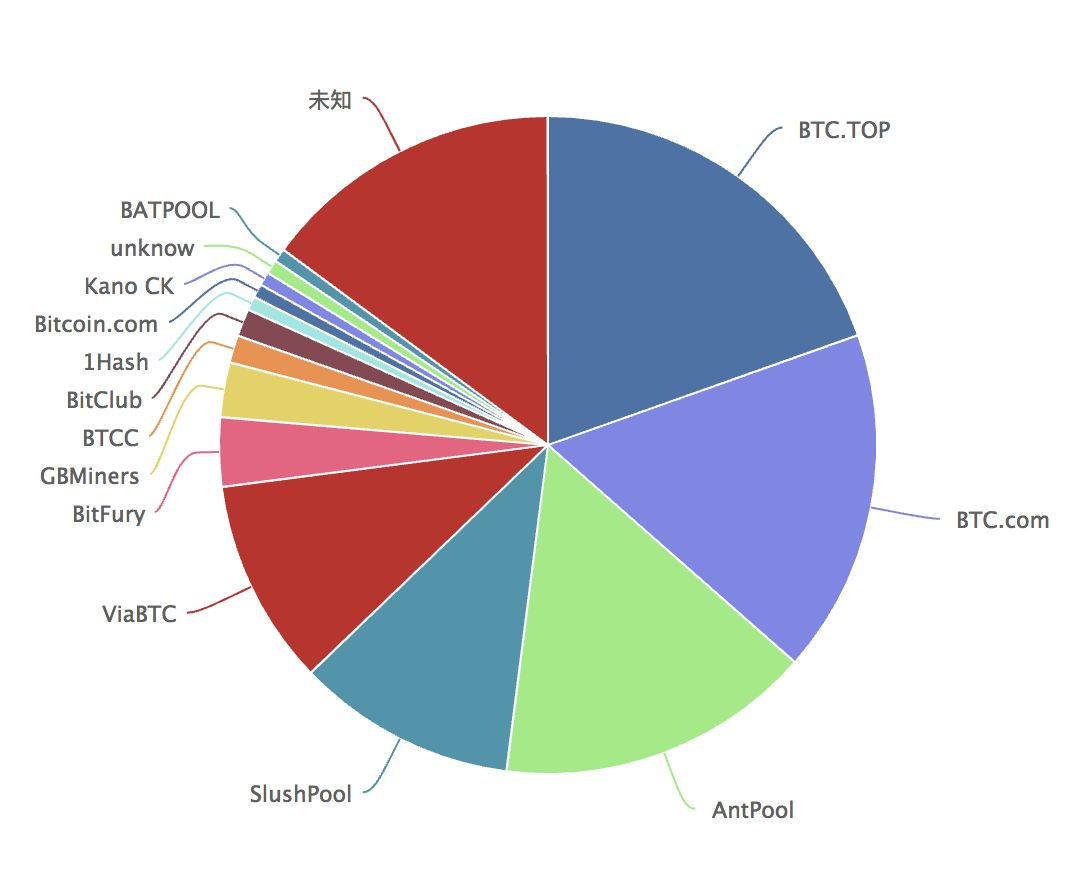
\includegraphics[width=0.45\linewidth]{figures/poolPie}
		\caption{前三公有矿池如果被操纵就具备超过51\%的算力\footnote{51\%攻击揭示了超过50\%的算力被恶意用户操纵的话比特币的记录就存在被操纵和篡改的风险。}。}
			\label{fig:poolpie}
		\end{figure}
		
\end{frame}

\subsection{比特币矿场}

\begin{frame}{全球加密货币矿场分布图}
	比特币矿场7成来自中国,其中4成在四川(2017年数据)。
	\begin{figure}
		\centering
		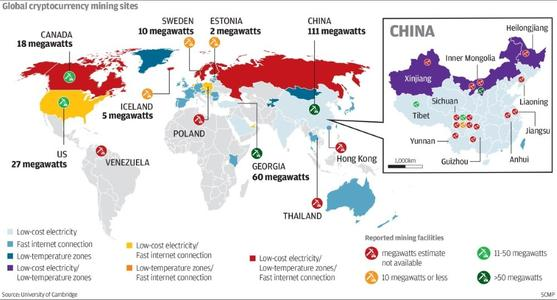
\includegraphics[width=0.9\linewidth]{figures/globalCryptocurrencyMiningMap}
		\caption{全球加密货币挖矿分布图}
		\label{fig:globalcryptocurrencyminingmap}
	\end{figure}
\end{frame}

\begin{frame}{矿场实景图}
	\begin{figure}
	\centering
	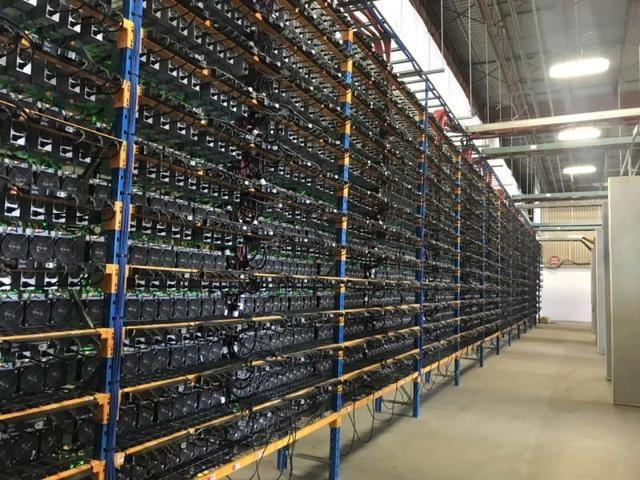
\includegraphics[width=0.7\linewidth]{figures/miningFactory}
	\caption{矿场内部的场景,密密麻麻的矿机}
	\label{fig:miningfactory}
	\end{figure}
\end{frame}

\begin{frame}{比特币挖矿能耗惊人}
	\begin{figure}
		\centering
		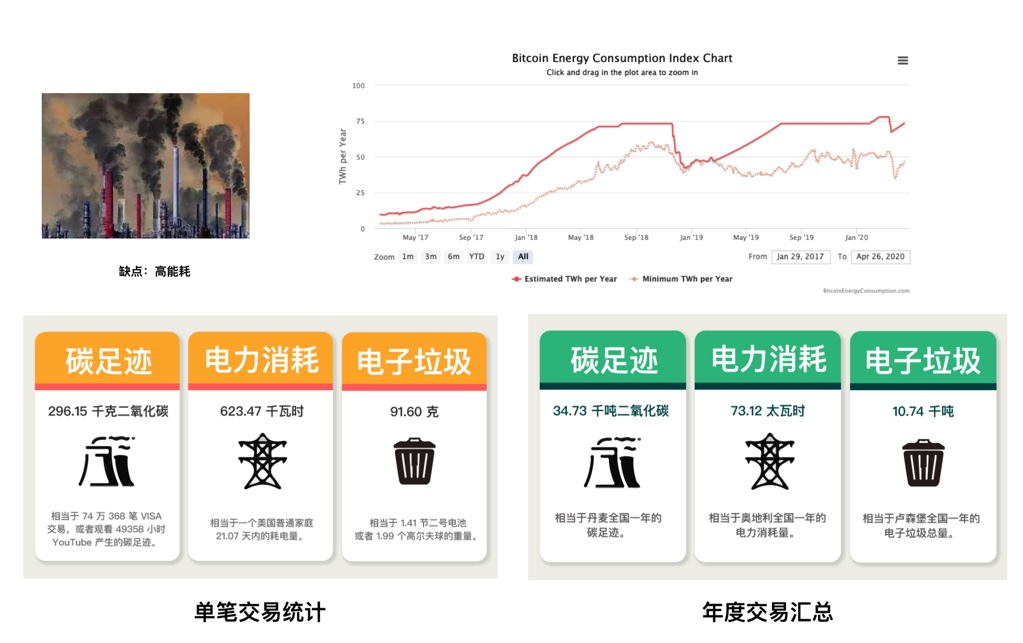
\includegraphics[width=0.88\linewidth]{figures/powerWastedOfBTCjpg}
		\label{fig:powerwastedofbtcjpg}
	\end{figure}
	
\end{frame}
\subsection{从面对面到交易所到数字货币信用卡}
% 面对面交易至交易所
\begin{frame}{面对面交易}
	内容...
\end{frame}

\begin{frame}{交易所}
	提供了数字货币价格展示、加密货币间交易、加密货币衍生品交易
	\begin{itemize}
		\item 币币交易;
		\item OTC交易;
		\item 去中心化交易所;
		\item 平台币;
	\end{itemize}
\end{frame}

\begin{frame}{加密货币信用卡、ATM}
	
	\begin{minipage}[t]{0.5\linewidth}
		\centering
		\begin{enumerate}
			\item 加密货币信用卡可以在日常消费中使用加密货币进行支付;
			\item 加密货币ATM可以使用加密货币兑换现金,或进行加密货币的转账等;
			\item 澳洲、欧洲对加密货币信用卡、ATM支持度较高。
		\end{enumerate}
	
	\end{minipage}%
	\begin{minipage}[t]{0.4\linewidth}
		\begin{figure}
			\centering
			\subfigure[加密货币信用卡]{
				\begin{minipage}[b]{0.8\linewidth}
					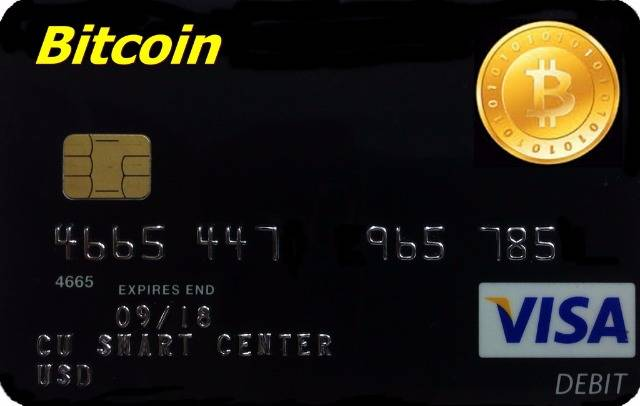
\includegraphics[width=\linewidth]{figures/btcVisaCard}
				\end{minipage}%
			}
			\subfigure[加密货币ATM]{
				\begin{minipage}[b]{0.8\linewidth}
					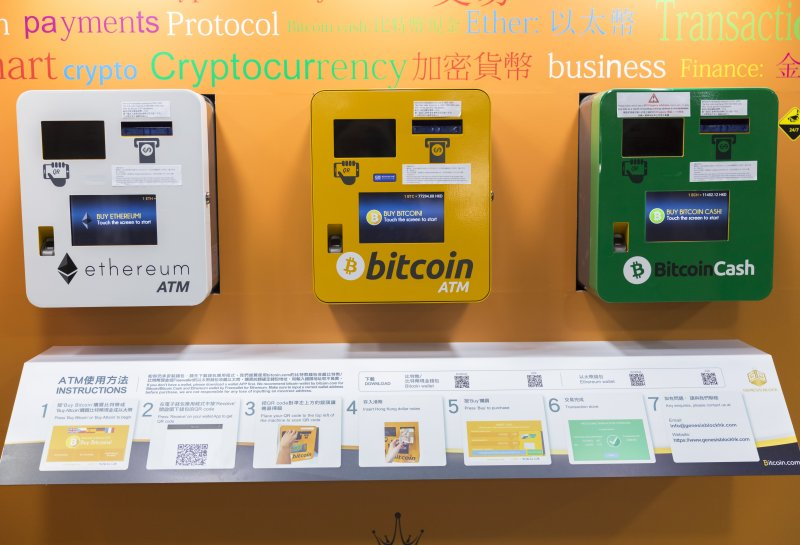
\includegraphics[width=\linewidth]{figures/bitcoinAtm}
				\end{minipage}%
			}
		\end{figure}
	\end{minipage}%
\end{frame}

\subsection{比特币金融衍生品}

\begin{frame}{常见比特币金融衍生品}
		\begin{minipage}[t]{0.7\linewidth}
		\footnotesize
	\begin{enumerate}
	\item 期货类:期货合约是期货交易所制定的标准化合约,对合约到期日及其买卖的资产的种类、数量、质量作出了统一规定。
	\begin{enumerate}
		\item 火币、OkEx、BitMEX等从交割合约的基础上衍生出永续合约;
		\item 芝加哥商品交易所CME和芝加哥期权交易所CBOE等;
	\end{enumerate}
	\item 期权类:期权交易是买卖权利的交易。期权合约规定了在某一特定时间、以某一特定价格买卖某一特定种类、数量、质量原生资产的权利;
		\begin{enumerate}
		\item 芝加哥商品交易所CME推出比特币期权;
	\end{enumerate} 
	\item 去中心化金融 DiFi:区块链和智能合约设计金融产品;
	\item 稳定币;
\end{enumerate}
	\end{minipage}%
	\begin{minipage}[t]{0.3\linewidth}
	\begin{figure}
		\centering
		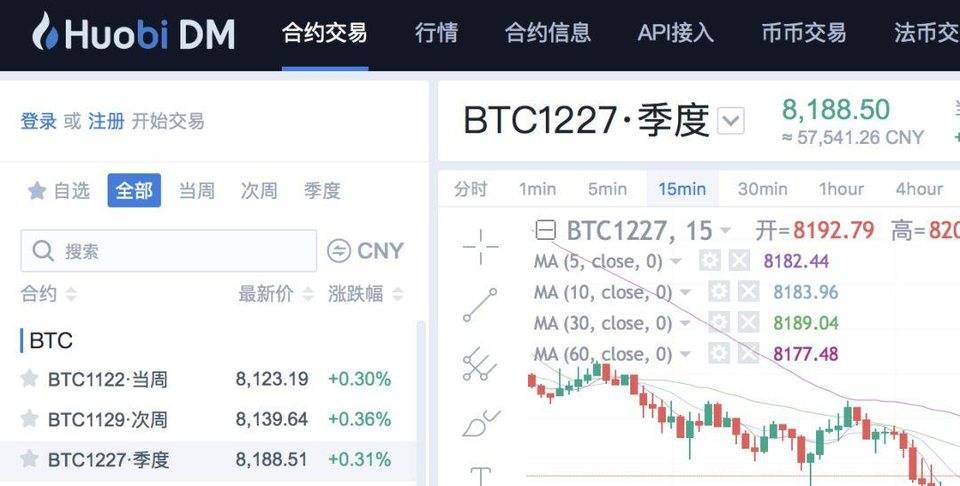
\includegraphics[width=\linewidth]{figures/ccContracts}
		\caption{火币合约交易截图}
	\end{figure}
	\end{minipage}%
\end{frame}

\section{智能合约和ICO狂潮}
\subsection{智能合约对区块链的意义}
\begin{frame}{智能合约定义}
	智能合约是一种特殊协议,在区块链内制定合约时使用,当中内含了程式码函式,亦能与其他合约进行互动、做决策、储存资料及传送加密货币等功能。
	
	提出者:尼克·萨博(Nick Szabo)1995年
\end{frame}

\begin{frame}{智能合约对区块链的意义}
	\begin{enumerate}
		\item 
	\end{enumerate}
\end{frame}
\subsection{区块链的ICO狂潮和百家争鸣}
\subsection{DAPP爆发和ICO狂潮}

\section{区块链脱虚向实}
\subsection{各国出台区块链政策密集出台}
\subsection{中国各省区块链政策密集出台}
\subsection{区块链应用领域一览}

\section{区块链历史经验总结}

\begin{frame}{勿当韭菜!!!别碰加密货币!!!}
	
	{\color{red}
		数字货币骗子口头禅大赏:
		\begin{itemize}
			\item 发币前许你美景:MIT、JP摩根团队;价值投资;一币一别墅;
			\item 发币后叫你稳住:团队在做事;拿住;价值投资;
		\end{itemize}
	}
	\begin{figure}
		\centering
		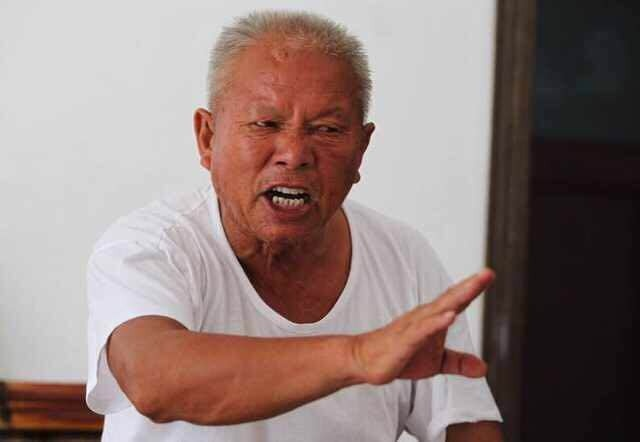
\includegraphics[width=0.5\linewidth]{figures/AllInGrandpa}
		\caption{什么团队背景,什么技术方案,老夫选币都是一把梭.mp4}
		\label{fig:allingrandpa}
	\end{figure}
	
\end{frame}

\end{document}